%%%%%%%%%%%%%%%%%%%%%%%%%%%%%%%%%%%%%%%%%%%%%%%%%%%%%%%%%%%%%%
%% Use this for a a4 output
%\documentclass
[
	paper=a4,
	fontsize=11pt,
	headings=big,
	parskip,
	numbers=noendperiod, % 2.3.1 vs 2.3.1. (no dot after the last chapter number)
	twoside=true,
	headinclude,
	pagesize,
	headsepline,
	toc=bibliography, % Bibliography appears in Table of Contents (without a number)
	version=last % Use latest version of the KOMA-Script
]
{mttTemplate}
\usepackage[twoside,bindingoffset=6mm]{geometry}
\setlength{\headsep}{2.5em}

%% allows for conditioning on the paper format
\providetoggle{a4style}
\settoggle{a4style}{true}

%% Use this for your booklet
\documentclass
[
	paper=b5,
	fontsize=11pt,
	headings=big,
	numbers=noendperiod, % 2.3.1 vs 2.3.1. (no dot after the last chapter number)
	twoside,
	paper=17cm:24cm,
	DIV=14,
	BCOR=5.0mm,
	parskip=half, %% better paragraph spacing
	cleardoublepage=empty,
	headinclude,
	pagesize,
	headsepline,
	toc=bibliography, % Bibliography appears in Table of Contents (without a number)
	version=last % Use latest version of the KOMA-Script
]
{mttTemplate}

\usepackage{geometry}
\geometry{ignoreall,heightrounded}

\setlength{\headsep}{2.5em}

%% allows for conditioning on the paper format
\providetoggle{a4style}
\settoggle{a4style}{false}

\flipbindingmargins
%%%%%%%%%%%%%%%%%%%%%%%%%%%%%%%%%%%%%%%%%%%%%%%%%%%%%%%%%%%%%%

%% Add the configuration and packages
%% Use this document for your meta data definitions.
%% These definitions can subsequently be used as \mtt<option>, for example: \mttAuthor

\newcommand\thesisauthor{Robbert Harms}
\newcommand\thesisauthorfull{Robbert Leonard Harms}
\newcommand\thesistitle{Maastricht Thesis Template v2}
\newcommand\thesisyear{2050}
\newcommand\thesisdate{2050-01-01} % or set to \today for the day of compilation.

% The date at which you will defend your thesis
\newcommand\thesisdefendingdate{Thursday 9th of June 2050} 
\newcommand\thesisdefendingtime{14.00 hours} 

\newcommand\thesispromotors{
Prof. Dr. Strange
}
\newcommand\thesiscopromotors{
Dr. Who
}
\newcommand\assessmentcommittee{
...
}

\newcommand\coverdetails{Robbert Harms, 2019}
\newcommand\productiondetails{Harms 2019, $\vert\vert$ Publisher Harms Press}
\newcommand\isbnnumber{xxx-xxxx-xxx-xx-x}
%%% Defines the packages for your thesis will be using

%% The font used
\usepackage{palatino}
%% For some fake text, can be removed if you have some content 
\usepackage{blindtext}
\usepackage{lipsum}  
\usepackage{afterpage}
%% For adding illustrations and graphics
\usepackage{graphicx}

%% better urls in bibliography
\usepackage[hidelinks]{hyperref}
%% a workaround for all texttt and urls that cross the borders
{\setlength\emergencystretch{3cm}

%% better looking tables by default
\usepackage{booktabs}

%% a different table class
\usepackage{tabularx,ragged2e}
\newcolumntype{C}{>{\Centering\arraybackslash}X} % centered "X" column
\newcolumntype{L}{>{\arraybackslash}X} % left aligned "X" column

%% allows you to rotate figures and tables
\usepackage[figuresright]{rotating}

%% for using things like \mathbb
\usepackage{amssymb}

%% for other math environments
\usepackage{amsmath}
\DeclareMathOperator*{\argmin}{argmin}
\DeclareMathOperator{\arctantwo}{arctan2}

%% for automatically breaking equations over lines
\usepackage{breqn}

%% for hyphenation of works already containing an hyphen
%% use \hyp{} in those words, e.g. Levenberg\hyph{}Marquardt
\usepackage{hyphenat}

%% for more advanced appendices
\usepackage{appendix}

%% for referencing things by name
\usepackage{nameref}

%% for better units support
\usepackage{siunitx}

%% For tables using more than one page
\usepackage{ltablex}

%% Cells spanning multiple rows in the tables
\usepackage{multirow}

%% Avoid putting floats in the next section
\usepackage[section]{placeins}

\usepackage{graphicx}

%%%%% Chapter 2 %%%%%
\usepackage{caption}
\usepackage{subcaption}
\usepackage{float}

\usepackage[justification=centering]{caption}
\usepackage{longtable}
\usepackage[format=plain,labelfont={it},textfont=it]{caption}

\usepackage{lscape}
\usepackage{adjustbox}
\usepackage{comment}

%%%%% chapter 4 %%%%%

\usepackage{mathtools}
\usepackage{cuted}

\raggedbottom

%%%% chapter 5 %%%%%
\usepackage{amsthm}

\usepackage{rotating}
\usepackage{tikz}

%%%%% chapter 7 %%%%% 
\usepackage{soul}
\usepackage{algorithmic}
\usepackage{textcomp}
\usepackage{listings}
\usepackage{xcolor}
\usepackage{url}

\usepackage{wrapfig}
%% This can be used to give hints to latex on where it can place hyphenations at line-breaks.
%% Just add new elements with space as separators. To disable hyphenation for a word just spell 
%% it out without dashes.
\hyphenation{hy-phe-na-tion}

%% Path to the directory containing the graphics and figures
%% You can add more subpaths by adding ``,{./figures/subdir/}`` within the first set of brackets.
\graphicspath{{./figures/}}

%% Load the default bibliography file
\addbibresource{bibliography.bib}


%% handy websites:
%% https://www.tablesgenerator.com/
%% https://www.codecogs.com/latex/eqneditor.php


\begin{document}
\UseRawInputEncoding
%% The front matter
\frontmatter
    \headerpage
    \thesistitlepage
    \infopage[true]  % set to false to disable the copyright text
    \dedication{To my parents and my grandparents}
    \tableofcontents

\urlstyle{same}
%% Start the main content
\mainmatter
	\chapter{Introduction}
\begin{refsection}
% [For writing - structure]
% \begin{itemize}
% \item how the data is being used, shared and analysed today?
% \item what is the data distribution situation today
% \item the need and benefits to share data and jointly analyse (discover potential knowledge and improve services... EU commission doc
% \begin{itemize}
% \item evidence / examples (global, EU, US, CN)
% \item  healthcare
% \item  climate 
% \item  social science
% \end{itemize}
% \item However, there are some challenges
% \begin{itemize}
% \item data is distributed - geographically, geographically, politically, regulation, technical...
% \item on national level?
% \item on organizational level
% \item on society level (legal, ethical societal)
% \item on individual citizen / data provider level 
% \end{itemize}
% \end{itemize}
\clearpage

\section{Section1}

The amount of data is growing every single day. The data produced globally is expected to be 175 zettabytes in 2025, growing dramatically from 33 zettabytes in 2018 ~\cite{european_commission_proposal_2020}. These massive amounts of data are used to improve digital technologies and develop data-driven innovations that can impact every aspect of people's lives ~\cite{european_commission_directorate_general_for_communications_networks_content_and_technology_study_2021}...

\printbibliography[heading=subbibintoc]
\end{refsection}


	\chapter{My second paper}
%% full citation of a work on the title page
\papercitation{MTTHarms2019}
\clearpage

\section*{Abstract}
Abstract here.

\cleardoublepage

\section{Introduction}
\lipsum
	\chapter{A Privacy-Preserving Infrastructure for Analyzing Personal Health Data in a Vertically Partitioned Scenario}

%% full citation of a work on the title page
\papercitation{sun_medinfo_2019}
\clearpage

\begin{refsection}
\section*{Abstract}Abstract
\section{Introduction}

\cleardoublepage

% \printbibliography[heading=subbibintoc]
\end{refsection}
	\chapter{Studying the Association of Diabetes and Healthcare Cost on Distributed Data}
%% full citation of a work on the title page
\papercitation{sun2022vwdata}
% \papercitationChaFour
\clearpage

\begin{refsection}
\section*{Abstract}
Abstract
\section{Introduction}

\clearpage



\end{refsection}
	\chapter{Privacy-Preserving Generalized Linear Models on Vertically Partitioned Data using Distributed Block Coordinate Descent}
%% full citation of a work on the title page

\papercitationChaFive{}
\clearpage

\begin{refsection}
\UseRawInputEncoding
\section*{Abstract}Abstract.

\cleardoublepage

\section{Introduction}
With technological developments in computational power and storage capacity, an increasing amount of data is collected and stored by a variety of data parties~\cite{kaisler2013big}....


\end{refsection}
	\chapter{Generating Synthetic Tabular Data using Conditional GANs combining with Differential Privacy}
%% full citation of a work on the title page
% \papercitation{}
\papercitationChaSix
\clearpage
\newcommand{\dpcgans}{DP-CGANS}

\begin{refsection}
\section*{Abstract}Abstract

\cleardoublepage

\section{Introduction}
\label{intro}
Data from individuals such as personal health or behavior data have proven to be highly valuable for health research such as enhancing our understanding of disease and delivering high-quality patient-centered care~\cite{nass2009value,kalkman_patients_2022}. ...


% \printbibliography[heading=subbibintoc]
\end{refsection}
	\definecolor{codegreen}{rgb}{0,0.6,0}
\definecolor{codegray}{rgb}{0.5,0.5,0.5}
\definecolor{codepurple}{rgb}{0.58,0,0.82}
\definecolor{backcolour}{rgb}{0.95,0.95,0.92}
\lstdefinestyle{mystyle}{
    backgroundcolor=\color{backcolour},
    belowcaptionskip=1\baselineskip,
    showstringspaces=false,
    basicstyle=\footnotesize\ttfamily,
    commentstyle=\itshape\color{green!40!black},
    identifierstyle=\color{blue},
    stringstyle=\color{orange},
}
\lstset{style=mystyle, columns=fullflexible}


\newcommand{\tidal}{TIDAL}
\chapter{ciTIzen-centric DatA pLatform (\tidal): Using Distributed Personal Data in a Privacy-Preserving Manner for Health Research}
%% full citation of a work on the title page
\papercitationChaSeven
\begin{refsection}

\clearpage

\section*{Abstract}Abstract
\clearpage

\section{Introduction}
\label{sec:introduction}
Giving individuals more control over who can access their personal data for what purpose and to make their data available using privacy-preserving and transparent methodologies will significantly encourage their engagement in health research~\cite{chen2016personalized,hulsen2020sharing}...

\printbibliography[heading=subbibintoc]
\end{refsection}
	\chapter{Discussion}
	


%%% \chapter{Conclusion}
\clearpage
% I would restate the main thesis 
% and that it has/has not been achieved, 
% secondly, the related considerations outlined in the discussion, 
% and finally a statement about the future.
 # integrated in discussion chapter	


%% The final part of the book, the bibliography and final parts
\backmatter	
    %% for the "notcategory" see the mttTemplate.cls file
% 	\printbibliography[notcategory=ignore]
	
	\chapter{Summary}
This is for the English summary of your work.
	\chapter{Samenvatting}
 %% TO DO %%
	\chapter{Valorisation}
How does this work benefit society? %% TO DO %%
	\chapter{Acknowledgments}


	\chapter{List of manuscripts}

%% if you want to ignore this publication in the Bibliography section
%\addtocategory{ignore}{myself2020}

%% Inserts a full citation of a bib reference
% \textbf{Published work:}
\begin{small}
\textbf{Published:}


\fullcite{sun_medinfo_2019}

\fullcite{van2018using}

\fullcite{sun_systematic_2021}

\fullcite{wouters2021putting}

\fullcite{houbraken2017discovering}

\fullcite{choudhury2022privacy}

\fullcite{Sun2019TransformationAI}

\fullcite{sun2022fairassess}

\fullcite{sunprivacy}

\fullcite{sun2022vwdata}

\textbf{Submitted/Pre-printed:}

\fullcite{van2019privacy}

\fullcite{sun2021knowledge}

\fullcite{eigenschink2021deep}


\fullcite{sun_syndata_2022}

\fullcite{sun_tidal_2022}

\fullcite{solid_privacy}
\end{small}



	\chapter{About the author}

\begin{wrapfigure}[18]{r}{0.45\textwidth}
  \begin{center}
    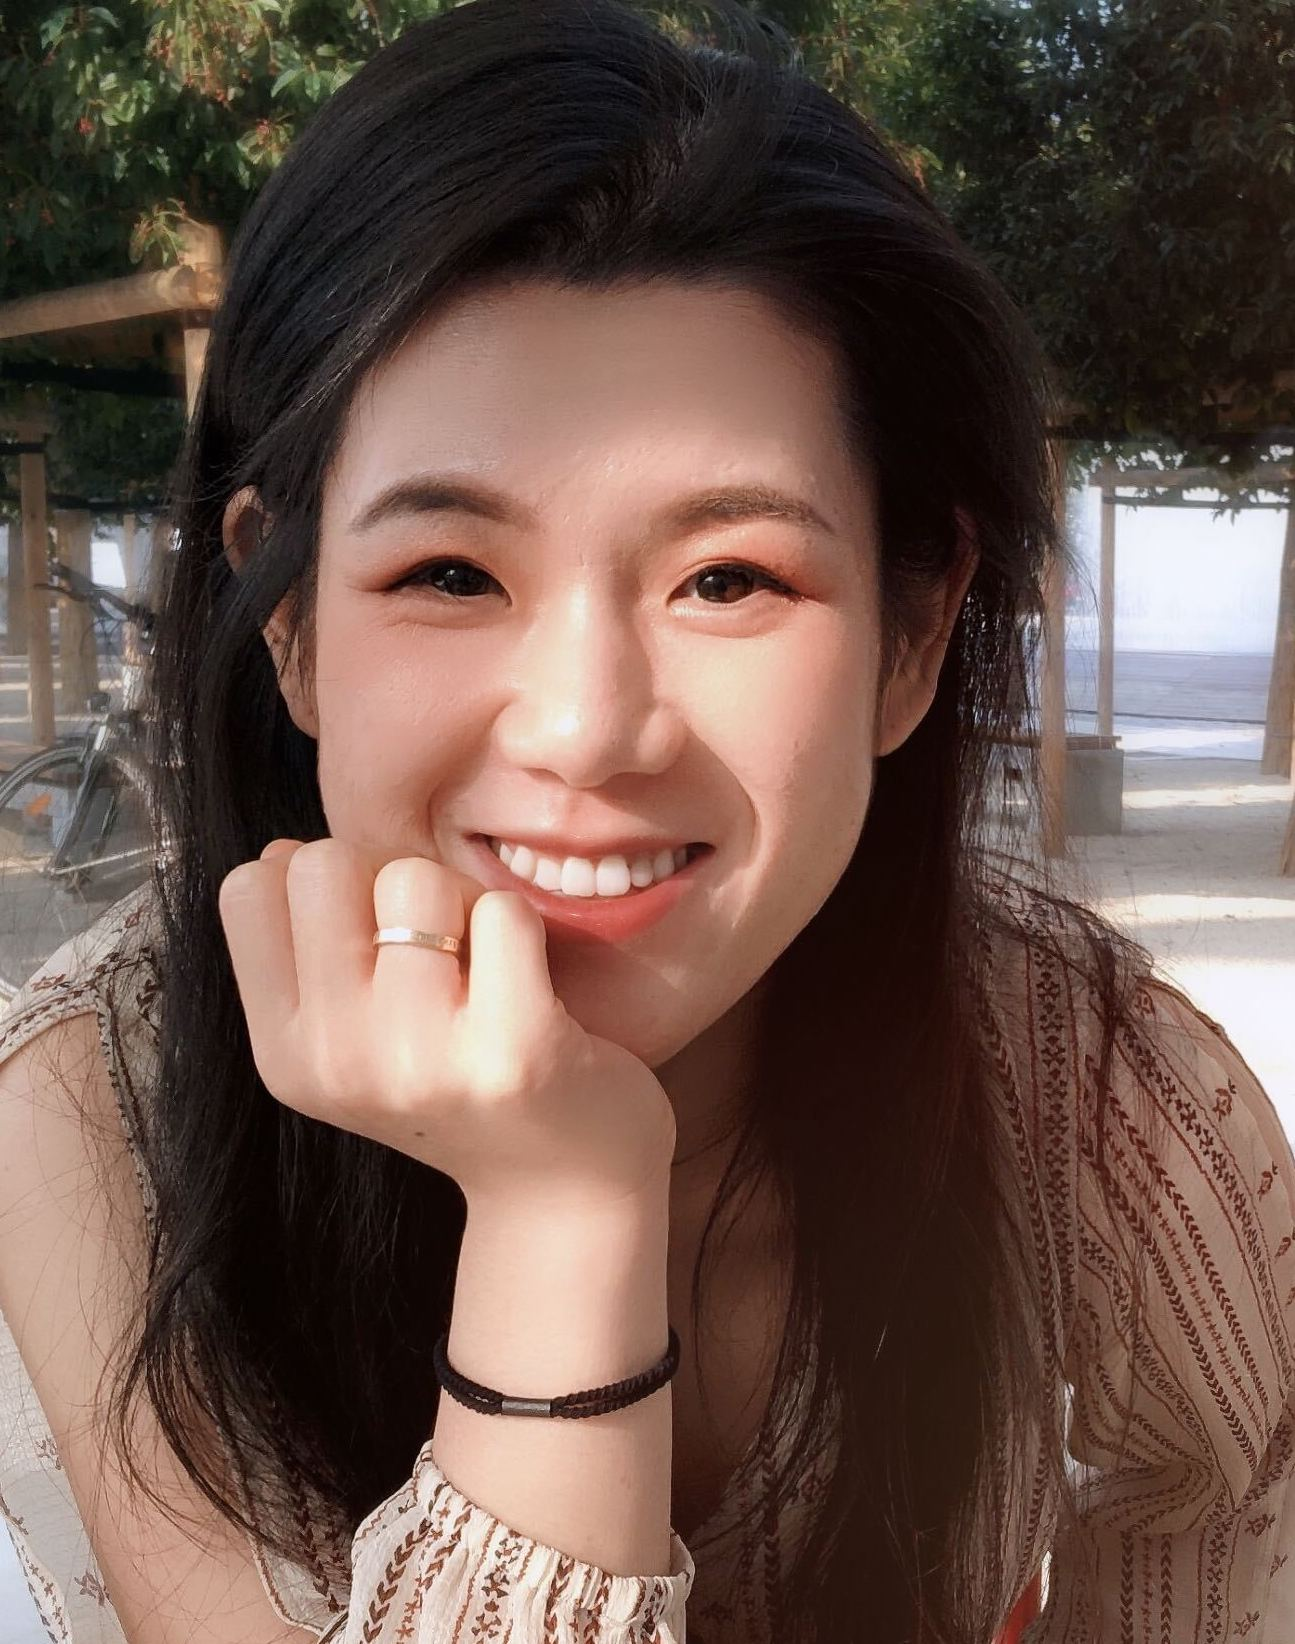
\includegraphics[width=0.4\textwidth]{img/chang_profile.jpg}
    % \vspace{-10pt}
  \end{center}
\end{wrapfigure}



  

\end{document}